\documentclass[xcolor=dvipsnames]{beamer}
\usepackage[ngerman]{babel}
\usepackage[orientation=portrait,size=a0]{beamerposter} %2378 x 1682
\mode<presentation>{%
%  \usetheme{Frankfurt}%
}

\usepackage{mwe}
\usepackage{tikz}
\usetikzlibrary{decorations.pathreplacing,angles,quotes}

\usepackage{subfigure}
\usepackage{graphicx}  % remove 'demo' option for your real document
\usepackage{caption}
\captionsetup[figure]{labelformat=empty}% redefines the caption setup of the figures environment in the beamer class.

\usepackage[round, comma, sort&compress]{natbib}

\usepackage{hyperref}
\hypersetup{urlcolor=blue, colorlinks=true,  citecolor=blue} % Colors hyperlinks in blue - change to black if annoying
\definecolor{myblue}{rgb}{0.063, 0.176, 0.341}

\setbeamercolor{title}{fg=White,bg=myblue}
\setbeamercolor{frametitle}{fg=Blue,bg=Blue!20}
\setbeamercolor{block title}{fg=Blue,bg=Blue!20}
\setbeamercolor{section in head/foot}{bg=Blue}
\setbeamercolor{author in head/foot}{bg=Blue}
\setbeamercolor{date in head/foot}{fg=Blue}


\title[S. N. A. E. L.]
{
\parbox{.25\textwidth}{
\includegraphics[height=6cm]{UPLogo.png}\hfill}%
\parbox{.5\textwidth}{\centering \huge Frühwarnung vor Vulkanausbrüchen\hfill}%
\parbox{.23\textwidth}{\hfill
\includegraphics[height=6cm]{InstitutLogo.png}}%
}
\author{\centering\Large Prof. Dr. Eva Eibl (eva.eibl@uni-potsdam.de) \hfill}
\institute{\centering\Large Institut für Geowissenschaften, Universität Potsdam\hfill%
%\\An Col\'aiste Ollscoile, Baile \'Atha Cliath
}
\date{\centering\Large 11.Mai 2019 \\Potsdamer Tag der Wissenschaften \#PTDW}



\begin{document}

\begin{frame}[t]{}
\begin{beamercolorbox}{frametitle}
\maketitle
\end{beamercolorbox}
\vskip 5mm
  \begin{block}{\LARGE 1. Arten von Ausbrüchen}
  \begin{minipage}[t]{0.4\textwidth}
  \begin{figure}
    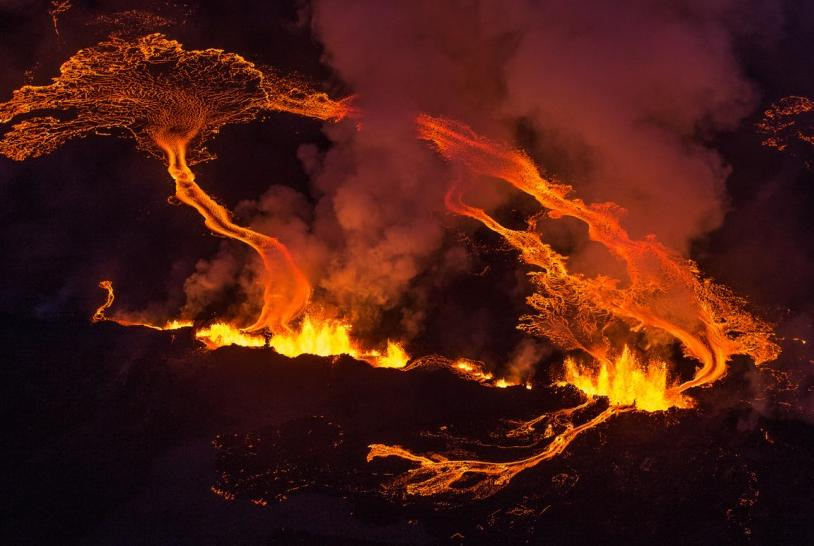
\includegraphics[scale=1.5]{images/1.jpg}
    \raggedright
      \captionsetup{justification=centering}
   	 \caption{\Large Effusiver Ausbruch\\ Holuhraun 2014/15, Island}
    \end{figure}
    \end{minipage}
    \hfill
  \begin{minipage}[t]{0.28\textwidth}
    \begin{figure}
      \centering
      \captionsetup{justification=centering}
    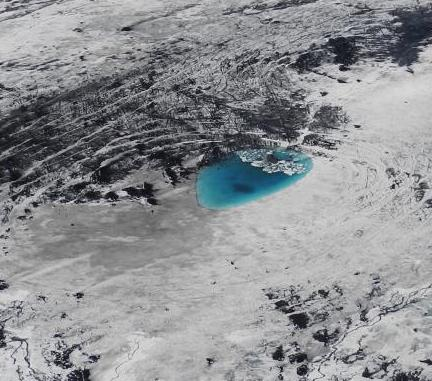
\includegraphics[width=26.5cm, height=21.5cm]{images/2.jpg}
    \caption{\Large Ausbruch unter einem Gletscher\\ Holuhraun 2014/15 Island}
     \end{figure}
     \end{minipage}
    \hfill
  \begin{minipage}[t]{0.3\textwidth}
    \begin{figure}
    \raggedleft
    \captionsetup{justification=centering}
    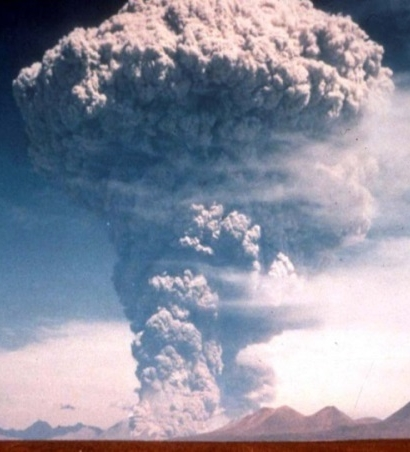
\includegraphics[width=20.5cm, height=21.5cm]{images/3.jpg}
      \caption{\Large Explosiver Ausbruch\\ Pinatubo 1991 Philippinen}
    \end{figure}
    \end{minipage}
  \end{block}
  
  \begin{minipage}[t]{0.385\textwidth}
  	\begin{block}{\LARGE 2. Vulkane global}
  \begin{itemize}
  \LARGE
  	\item 1508 Vulkane aktiv in letzten 10 000 Jahren 
	\item 10\% der Weltbevölkerung leben innerhalb 100 km Entfernung zu einem Vulkan
	\item $\sim$20-30 Ausbrüche zu jeder Zeit
  \end{itemize}
  \vskip 5mm
  \begin{figure}
  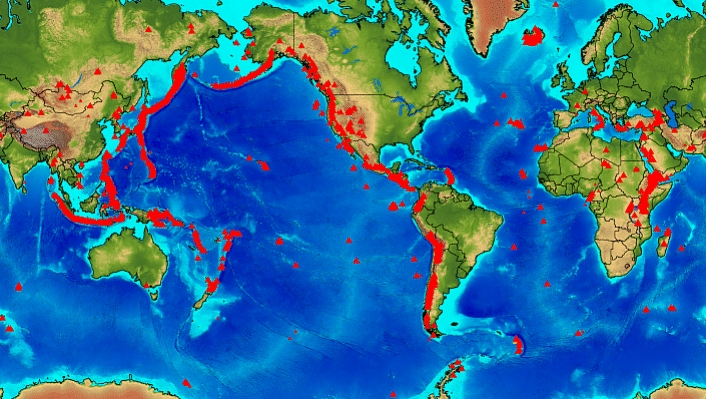
\includegraphics[trim=1cm 0cm 0cm 0cm, clip,height=26cm, width=32cm, angle=0]{images/4.jpg}
  \centering
      \captionsetup{justification=centering}
      \caption{\Large weltweite Verteilung von Vulkanen}
      \end{figure}       
  	\end{block}
  \end{minipage}
  \hfill
  \begin{minipage}[t]{0.6\textwidth}
  \begin{block}{\LARGE 3. Seismische Signale begleiten Vulkanausbrüche}
    \vskip 5mm
  		\begin{minipage}[h]{0.49\textwidth}
  		\begin{figure}
  		\begin{tikzpicture} 
  		\node[anchor=south west,inner sep=0] at (0,0){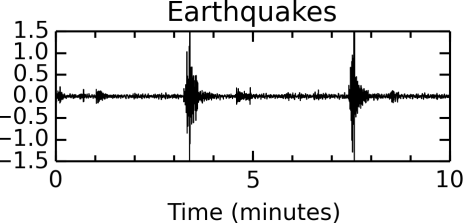
\includegraphics[scale=4.5]{images/5.jpg}};
  		 \node[fill=white] at (13.1,11.3) {\Huge Erdbeben   ~};
  		 \node[fill=white] at (13.1,0.7) {\LARGE Zeit (Minuten)   ~};
  		\draw[blue, decoration={brace,mirror,amplitude=30pt,raise=10pt},decorate]
  (10,6.5) -- node[right=50pt] {\LARGE Amplitude} (10,10);
  		 \end{tikzpicture}
  		 \end{figure}
  		\end{minipage}
  		\hfill
 		\begin{minipage}[h]{0.49\textwidth}
 		\begin{figure}
 		\begin{tikzpicture} 
  		\node[anchor=south west,inner sep=0] at (0,0){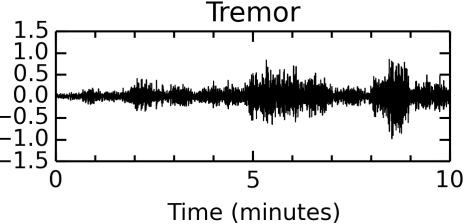
\includegraphics[scale=4.5]{images/6.jpg}};
  		 \node[fill=white] at (13.1,11.3) {\Huge Tremor   ~};
  		\node[fill=white] at (13.1,0.7) {\LARGE Zeit (Minuten)   ~};
 	 	 \draw[blue, decoration={brace,mirror,amplitude=40pt,raise=10pt},decorate]
  (12.5,6) -- node[below=35pt] {\LARGE Dauer} (17.5,6);
  		 \end{tikzpicture}
 		\end{figure}
	  	\end{minipage}
%\vskip 10mm
  \begin{figure}
  \begin{tikzpicture}
  \node[anchor=south west,inner sep=0] at (0,0) { 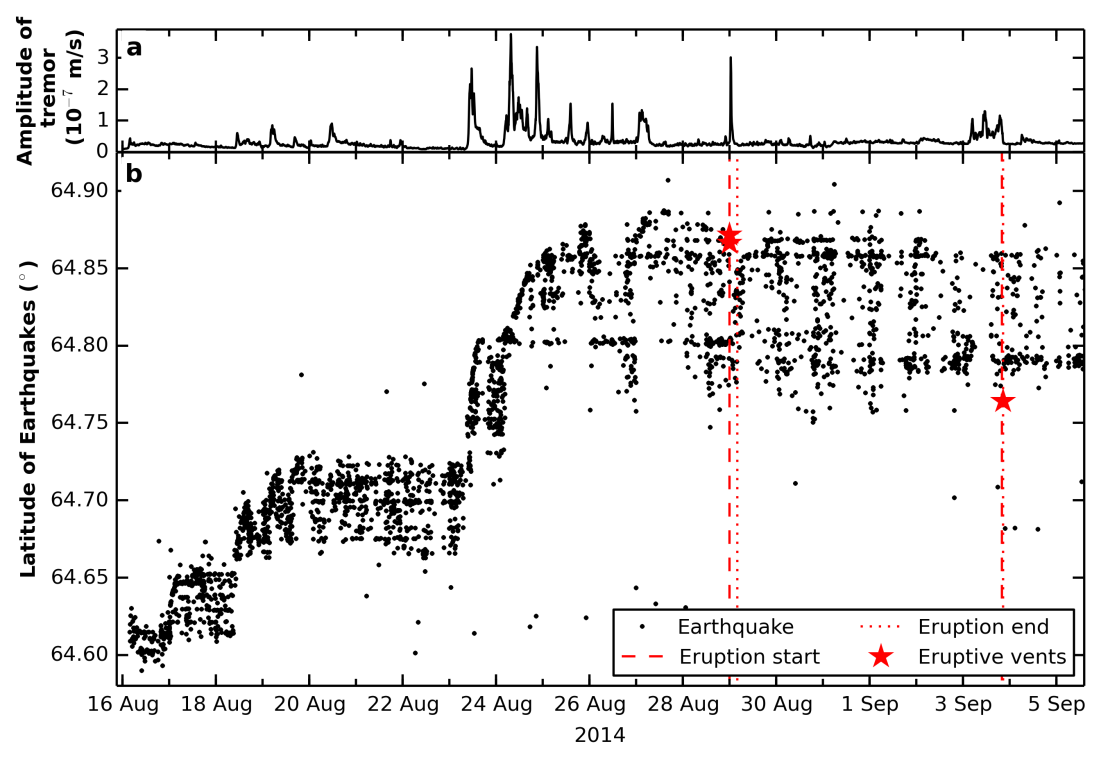
\includegraphics[width=49cm, height=21cm]{images/9.jpg}};
   
   \node[draw, red] at (32,16) {\Large Eruption außerhalb des Gletschers};
\node[draw, red] at (42,8) {\Large Eruption unter dem Gletscher};

\draw[blue, decoration={brace,mirror,amplitude=50pt,raise=50pt},decorate]
  (32.5,17) -- node[above=100pt] {\LARGE Vorboten} (5.5,17);
  
  \draw[blue, decoration={brace,mirror,amplitude=50pt,raise=30pt},decorate]
  (45,17) -- node[above=100pt] {\LARGE Vorboten} (43,17);
  
%\path pic ["$\theta$", draw, ->] {angle=pointx--O--point};  
   \end{tikzpicture}
   \centering
      \captionsetup{justification=centering}
   \caption{\Large zeitliche Entwicklung von Erdbebenherden, Bár$\eth$arbunga, Island. Nach \cite{Eibl2017b}}
   
  \end{figure}
 % \end{minipage}
%  
%  \begin{tikzpicture}
%  \node[anchor=south west,inner sep=0] at (0,0) { 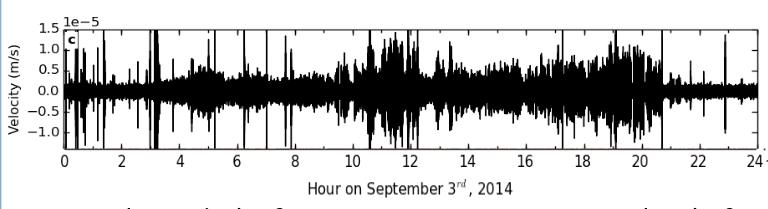
\includegraphics[trim=0.2cm 0cm 0cm 0.5cm, clip,scale=2.2]{images/7.jpg}};
%  \draw[red,ultra thick,rounded corners] (7.5,5.3) (5,9) -- (58,9);
%  \draw[black, decoration={brace,mirror,amplitude=50pt,raise=50pt},decorate]
%  (14,14.5) -- node[left=100pt] {\color{blue}\LARGE $Amplitude$} (14,9);
%   \end{tikzpicture}
%  
  \end{block}
  \end{minipage}
  \begin{block}{\LARGE 4. Wie sieht die Magmakammer aus und in welcher Tiefe liegt sie?}
  \vskip 5mm
  \begin{minipage}{0.27\textwidth}
  \begin{figure}
   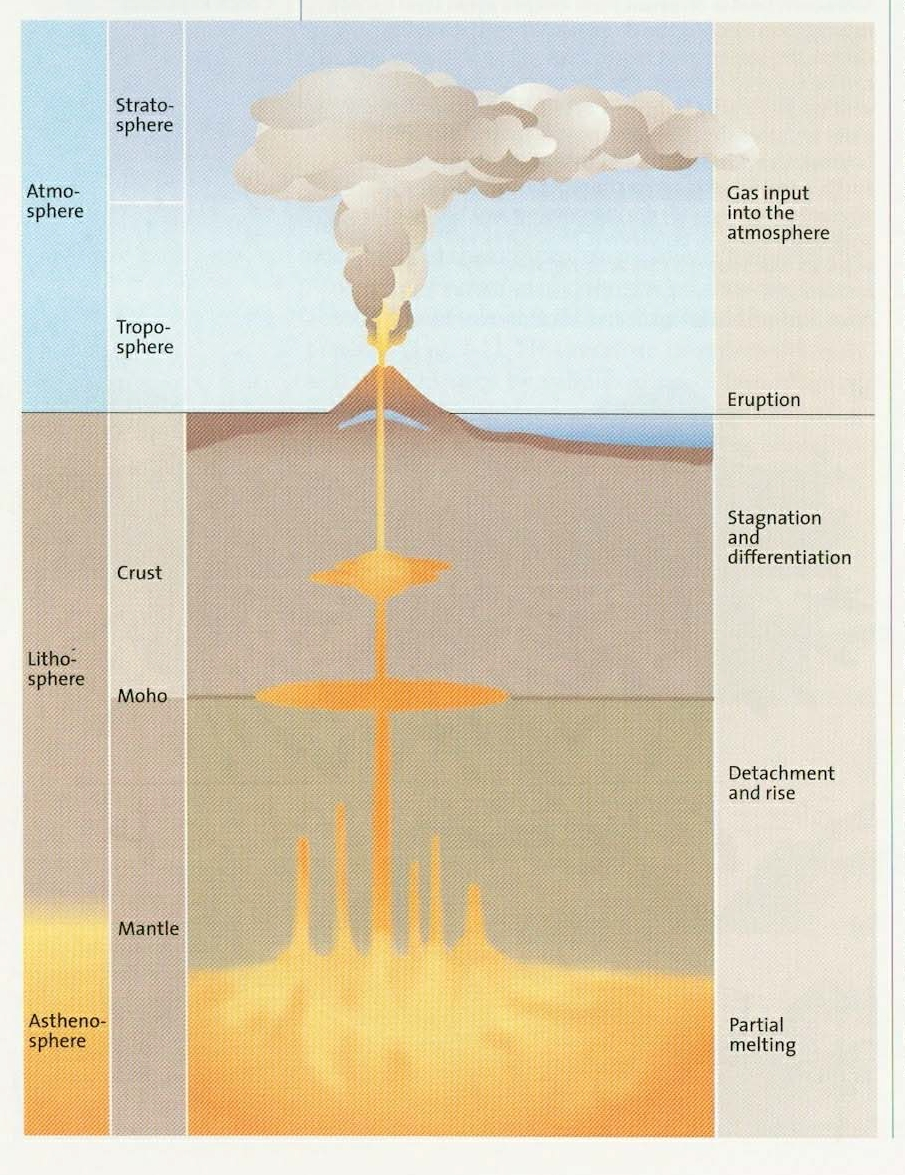
\includegraphics[scale=0.97]{images/8.jpg}
           \caption{\Large Schematischer Aufbau eines Vulkans}
   \end{figure}
  \end{minipage}
  \hfill
  \begin{minipage}{0.3\textwidth}
  \begin{figure}
   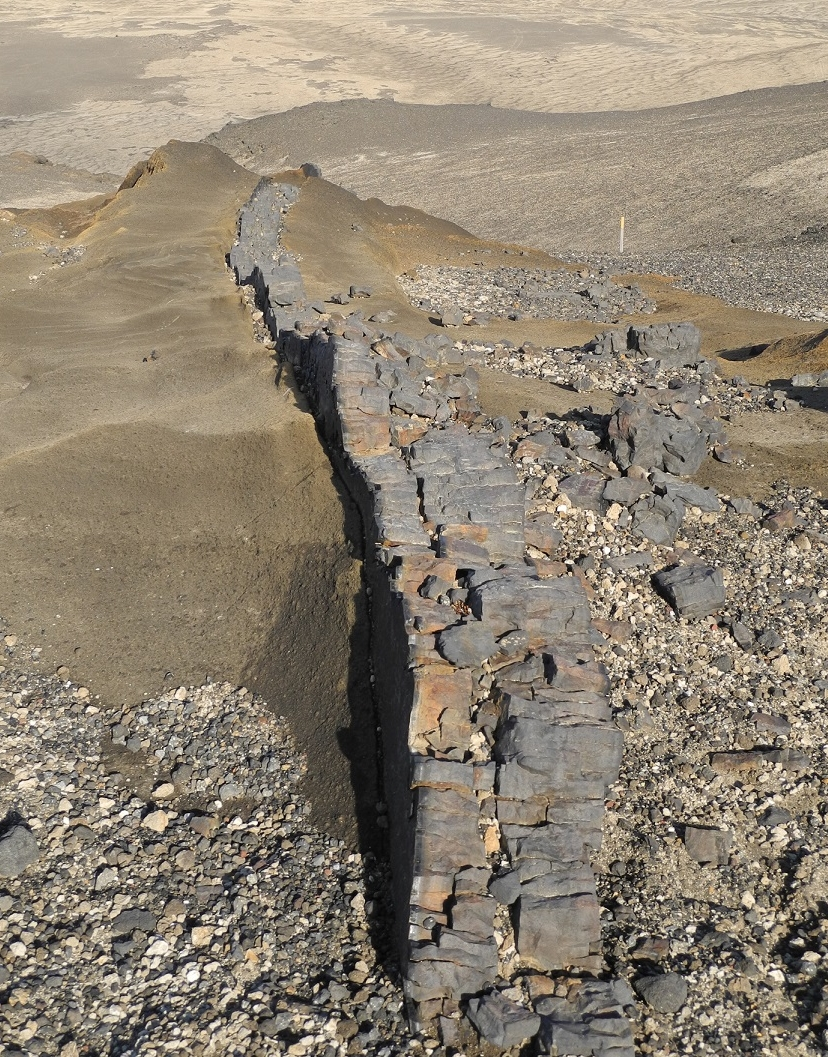
\includegraphics[scale=1.07]{images/10.jpg}
	\caption{\Large Magma Intrusion (Dyke)}
  \end{figure}
  \end{minipage}
     \hfill
  \begin{minipage}{0.42\textwidth}
  %\vspace{2mm}
  \begin{figure}
   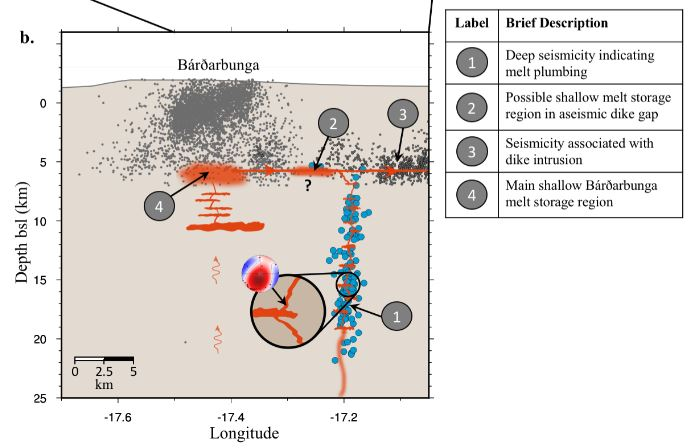
\includegraphics[scale=1.9]{images/12.jpg}
       \caption{\Large Arten vulkanischer Seismizität}
  \end{figure}
  \vskip -10mm
  \begin{block}{\LARGE Quellen}
	\begin{minipage}[h]{0.78\textwidth}
	\bibliographystyle{apa}%Used BibTeX style is unsrt
	\vskip 10mm
	\large
\bibliography{sample}
	\end{minipage}
	\hfill
	\begin{minipage}[h]{0.2\textwidth}
          
\includegraphics[scale=0.6]{images/11.jpg}
	\end{minipage}
  \end{block}
  \end{minipage}
      
  \end{block}
\end{frame}

\end{document}